\chapter{Problem Domain}

This chapter will describe the classes that is contained within the problem domain. The relations between the classes in the problem domain are described in \cref{sub:Structure}. The chapter aims to analyze the context of the system, with purpose of specifying the classes and the associated behaviors.

\section{Classes}
\label{sub:pd_classes}
These are the candidates for classes, the system needs to keep track of:
\begin{description}
    \item[Track]

    Used for storing meta data eg. artist, duration
    \item[User]

    Used for information about the user eg. votes
    \item[Vote]

    Which track a user voted for to be played, and when the vote was submitted.
    \item[Playlist]

    Used for keeping track of the votes and tracks
    \item[Restriction]

    To allow limitation of the set of tracks that can be added to the playlist.
    \item[Venue]

    To store information about the playlist and restrictions.
\end{description}

In order for the user to be able to vote for a track, a uniform way of referencing tracks is needed. This is done though a vote class that also contains the information about the vote; the user that voted, the track voted for and the time is was created. To achieve this, a catalogue is introduced. The user can then browse for a desired track.


\section{Structure}
\label{sub:Structure}
This section describes the relationships between the different classes
described in \cref{sub:pd_classes}. These relationships will be
visualised in a class diagram as described
in~\cite{mathiassen2001objektorienteret}.

The authors of~\cite{mathiassen2001objektorienteret} operate with three
main structuring techniques.

\begin{description}
\item[Generalisation] Generalisation is used to describe a \enquote{is-a}
  relationship between classes. A class is called a
  superclass when another class inherits attributes and operations
  from this superclass. The other class is now a subclass of the
  superclass. In class diagrams, generalisation is denoted by a
  triangular arrow pointing from the subclass to the superclass.
\item[Aggregation] Aggregation is used to describe a
  \enquote{contains} relationship between classes. In class diagrams,
  aggregation is denoted by a rhombus shaped arrow.
\item[Association] Association is used to describe that two classes
  are aware of each other. Association is denoted in class diagrams by
  a line between each class.
\end{description} \chnote{Hvorfor er det beskrevet?}

Based on these structuring techniques, a class diagram showing the structure of the classes in the problem domain of the system has been made. See \cref{fig:pd_structure}. Every \enquote{User} class has an association with either zero or one \enquote{Track} classes, i.e. they have voted on a track. A \enquote{Track} can have an association with an \enquote{Audio system} class in that it is currently being played. The \enquote{Playlist} class contains zero or more \enquote{Track} classes, i.e. the tracks yet to be played. A \enquote{Playlist} class has an association with a \enquote{Filter}, i.e. the playlist is filtered by a filter.

\begin{figure}
  \centering
  \includegraphics[width=\textwidth]{pd_structure.png}
  \caption{Class diagram of problem domain}\label{fig:pd_structure}
\end{figure}


\section{Behaviour}
\begin{figure}
  \centering
  \includegraphics[width=\textwidth]{StateDiagramDevice.jpg}
  \caption{Class diagram of problem domain}\label{fig:StateDiagramDevice}
\end{figure}

\begin{figure}
  \centering
  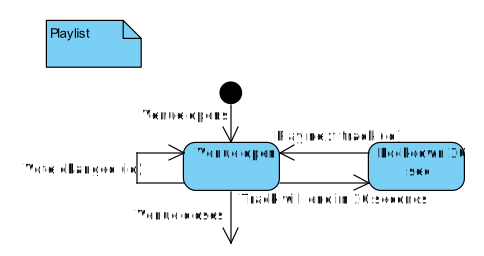
\includegraphics[width=\textwidth]{StateDiagramPlaylist.jpg}
  \caption{Class diagram of problem domain}\label{fig:StateDiagramPlaylist}
\end{figure}

\begin{figure}
  \centering
  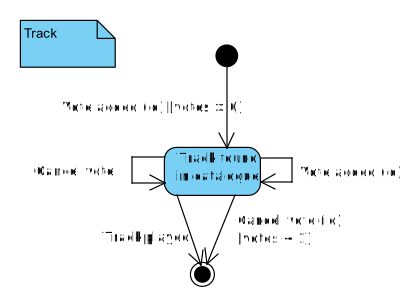
\includegraphics[width=\textwidth]{StateDiagramTrack.jpg}
  \caption{Class diagram of problem domain}\label{fig:StateDiagramTrack}
\end{figure}
